\documentclass[11pt]{article}
\usepackage[margin=1in]{geometry}
\usepackage{graphicx}
\usepackage{booktabs}
\usepackage{amsmath}
\usepackage{url}
\title{A Seeded Sensitivity Study of Utilization and Locality in a Simplified Page-Mapped Flash Simulator}
\author{Arnav Pandya}
\date{October 2026}
\begin{document}
\maketitle

\begin{abstract}
We measured page-program amplification in a small page-mapped flash translation layer simulator at three active logical-page utilizations (40\%, 70\%, 85\%) and under uniform or disjoint hot/cold update distributions. Across five matched pseudorandom seed blocks (30 condition runs), mean amplification for uniform traffic rose from 1.136 to 4.027 as utilization increased. For hot/cold traffic, means were 1.336, 1.835, and 2.244. The paired hot/cold-minus-uniform differences were +0.199 (95\% descriptive interval 0.186 to 0.213), -0.136 (-0.153 to -0.119), and -1.783 (-1.867 to -1.699), respectively. The interaction characterizes this allocator and synthetic workload; it is not a general property of NAND devices. The study provides a reproducible software sensitivity result, not a new FTL algorithm, hardware measurement, or SSD lifetime prediction.\\
\textbf{Keywords:} flash translation layer, write amplification, garbage collection, workload locality, simulation
\end{abstract}

\section{Introduction}
Flash translation layers map host logical addresses to physical NAND pages and reclaim invalid pages through garbage collection. Page relocation and erase-block reclamation make write amplification dependent on workload and device policy. Prior work has analyzed greedy collection, valid-page distributions, closed-form amplification, hot/cold policies, and locality-aware FTLs \cite{hu2009waf,agrawal2008design,bux2010greedy,peleato2012valid,agarwal2010closed,vanhoudt2013hotcold,chen2019hcftl,wang2015datacentric,kang2015hotpages,park2019model}. This paper evaluates only a compact educational model and asks: how do active logical-page utilization and update locality affect modeled program amplification and GC work under equal full-page overwrite semantics?

\section{Related Work}
Hu et al. analyze write amplification in flash-based SSDs, while Agrawal et al. describe mapping and garbage-collection trade-offs \cite{hu2009waf,agrawal2008design}. Bux and Iliadis analyze greedy collection performance, Peleato et al. characterize valid-page distributions under greedy GC, and Agarwal and Marrow derive a closed-form NAND amplification expression \cite{bux2010greedy,peleato2012valid,agarwal2010closed}. Research has also directly studied hot/cold data and garbage-collection algorithms, locality-aware page-level FTLs, data-centric collection, and policies based on hot-page ratios \cite{vanhoudt2013hotcold,chen2019hcftl,wang2015datacentric,kang2015hotpages}. Park et al. provide another write-amplification model \cite{park2019model}. Thus the broad premise that workload locality and utilization interact with garbage collection is established. The present result does not establish that its particular sign change is new: it is best treated as a reproducible characterization of this simulator under one synthetic workload design, not as an independent storage-systems principle.

\section{Simulation Architecture}
The simulator represents each physical page as free, valid, or invalid; logical-to-physical mappings reside in an in-memory dictionary. A host write programs one free physical page and invalidates a prior page for that LBA. When free pages approach the configured threshold, greedy GC chooses a block with many invalid pages, copies its remaining valid pages, and erases it. Ties favor a smaller erase count. The model excludes persistent mapping metadata, NAND timing, parallelism, bad blocks, ECC, failures, and static wear leveling. The supplied ring buffer packs record bytes but discards record LBAs; therefore it cannot be compared as an equivalent key-value store to direct writes.

\section{Experimental Methodology}
We used 16 blocks of 32 pages each (512 physical pages), a modeled page size of 4,096 bytes, and 5,000 full-page host overwrites per run. Active address spaces were rounded to 40\%, 70\%, and 85\% of physical-page count. Uniform runs sampled each active LBA uniformly. Hot/cold runs directed 80\% of updates to a hot range containing 10\% of active addresses and 20\% to a disjoint cold range containing the remainder. Five pseudorandom seeds (11, 23, 47, 89, 101) were reused across all six conditions, giving 30 condition runs arranged in five paired seed blocks. The generator uses common random numbers: latent draws are aligned by seed across conditions, while workload transformations and address sequences differ by condition. The five seed streams are the independent replication units for paired contrasts; the 30 condition runs are not 30 independent replicates of the interaction.

Let $H$ be host page programs and $G$ be valid-page GC copy programs. We report $A=(H+G)/H$, in modeled page-programs per host page-program. This excludes metadata and any internal device work. We also record erasures and per-block erase counts. Results combine startup and GC activity; run lengths were fixed and were not selected by a steady-state criterion. Cell means and sample standard deviations summarize the five seeds. We calculated paired hot/cold-minus-uniform differences within each seed and difference-in-differences across utilization levels; two-sided 95\% Student-$t$ intervals use four degrees of freedom. They describe between-seed variation for these fixed simulated conditions and are not population intervals for drives or real workloads.

\section{Results}
Table~\ref{tab:results} reports the trial means and standard deviations. Uniform workload amplification increased with utilization. Hot/cold amplification was higher at 40\%, but lower at 70\% and 85\%. Paired hot/cold-minus-uniform contrasts were $+0.199$ (40\%, 95\% descriptive $t_4$ interval $[0.186,0.213]$), $-0.136$ (70\%, $[-0.153,-0.119]$), and $-1.783$ (85\%, $[-1.867,-1.699]$). Difference-in-differences relative to 40\% were $-0.335$ ($[-0.350,-0.321]$) at 70\% and $-1.982$ ($[-2.060,-1.905]$) at 85\%. These estimates use five paired seed blocks; the intervals do not turn the six cells or 30 condition runs into independent interaction replications. Nor do they support inference to a population of devices or workloads. The pattern is conditional on this allocator, victim score, workload generator, and run length.

\begin{table}[ht]
\centering
\caption{Program amplification, mean $\pm$ sample SD across five seeds.}
\label{tab:results}
\begin{tabular}{@{}lrr@{}}\toprule
Utilization & Uniform & Hot/cold mixture \\\midrule
40\% & 1.136 $\pm$ 0.003 & 1.336 $\pm$ 0.013 \\
70\% & 1.971 $\pm$ 0.016 & 1.835 $\pm$ 0.011 \\
85\% & 4.027 $\pm$ 0.058 & 2.244 $\pm$ 0.041 \\\bottomrule
\end{tabular}
\end{table}

\begin{figure}[ht]
\centering
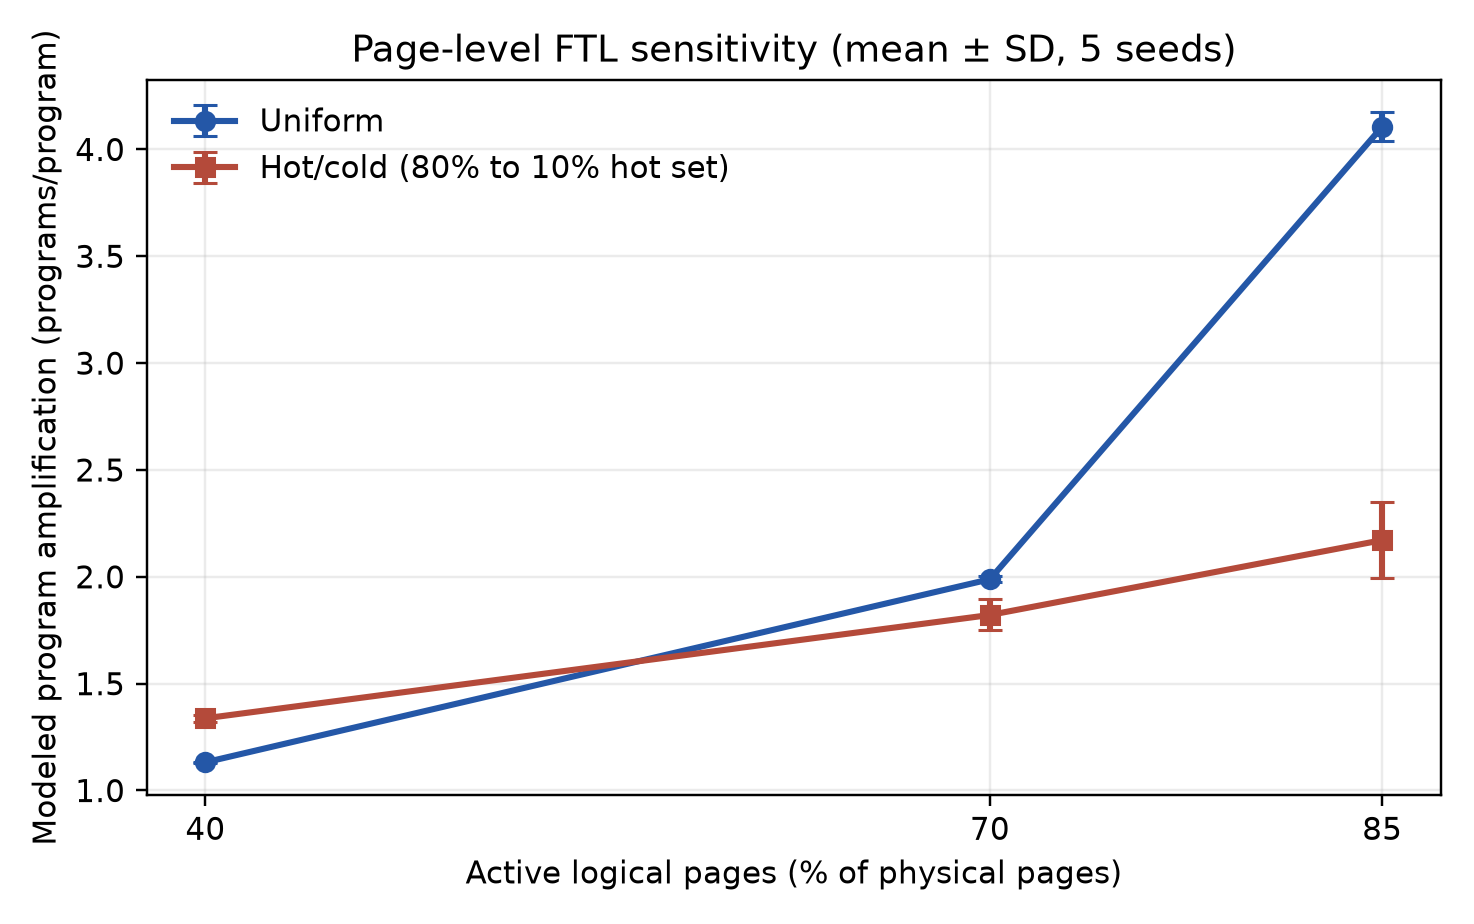
\includegraphics[width=0.82\linewidth]{../research/figures/program_amplification.png}
\caption{Modeled program amplification by active logical-page utilization. Error bars show one sample standard deviation across five seeds.}
\end{figure}

\section{Discussion}
The increase for uniform traffic at high utilization is consistent with fewer spare pages making reclamation more expensive in this model. The contrasting hot/cold trend indicates an interaction between locality, greedy victim selection, and allocation order for the chosen workload construction. Earlier studies already examine greedy GC and the effects of hot/cold data and locality-aware collection. Our observed reversal therefore cannot be presented as a novel general effect; its defensible value is as a transparent, repeatable result that exposes the behavior and limits of this particular implementation. Five seed blocks and one run length do not establish robustness to other workloads, geometries, or FTL algorithms. The outcome is a bounded simulator page-program ratio, not conventional device WAF validated against hardware.

\section{Limitations}
The simulator is a small abstraction, not a NAND model. It uses an in-memory mapping table and omits persistent recovery, controller caches, metadata writes, wear-leveling migration, timing, parallel channels, bad blocks, endurance failures, and hardware validation. Only six parameter cells, five seeds, and one run length were studied. The hot/cold mixture is not a canonical benchmark. Erase counts are simulated GC operations, not lifetime estimates. A previous 66-fold buffered/direct comparison is withdrawn because the buffered path did not preserve the same logical key-value state. Crash-loss outputs are queue occupancy accounting, not recovered-state durability results.

\section{Conclusion}
In this simplified page-mapped simulator, utilization and locality jointly affected modeled GC program amplification, with the locality ordering changing across utilization levels. The result is an educational, reproducible sensitivity study and corrected research-software artifact. It does not establish a general buffering benefit, a novel FTL technique, or predictions about commercial flash devices.

\section*{Code and Data Availability}
Source code, tests, experiment configuration, raw seeded trial outputs, and figure-generation scripts are available in the project repository at \url{https://github.com/apandya55/flash-waf-sim}. No archival DOI has been created. Reproduction commands are in \texttt{research/METHODOLOGY.md}.

\section*{AI Use Disclosure}
AI tools assisted with repository auditing, code editing, experiment scripting, and manuscript drafting. The author must verify all code, results, citations, and venue policies and revise this disclosure to match the target journal's current requirements.

\bibliographystyle{plain}
\bibliography{references}
\end{document}
